\section{Technische Realisierung}

\subsection{Architektur}
Das Projekt ist in folgende Module aufgeteilt:
\begin{itemize}
	\item EBP-Client
Grafisches Datenbankfrontend für den alltäglichen Gebrauch
	\item AdminDialog
Grafisches Datenbank-Administrationswerkzeug
	\item libEBPdb
Stellt Fachklassen und Persistenzfunktionen als Bibliothek zur Verfügung
	\item Unit-Tests
Automatisierte Tests der Bibliothek
\end{itemize}

\newpage

\subsection{Das QT-Framework}
\subsubsection{Grafische Oberfläche}\mbox{}\\
Die GUI wurde in grafischer Weise mit den bei QT mitgelieferten Tools erstellt.\\Diese Tools sind:
\begin{itemize}
	\item \textit{QT-Designer}\\[\baselineskip]der die grafisch erstellte GUI in XML-Form beschreibt und in \textit{U}ser \textit{I}nterface definition files (.ui) speichert.
	\item \textit{UIC} - \textit{U}ser \textit{I}nterface \textit{C}ompiler\\[\baselineskip]der die UI-Dateien liest und anschließend in C++-Header Dateien konvertiert.
\end{itemize}
\paragraph{UIC}\mbox{}\\
Der von \textit{UIC} generierte Code enthält das im QT-Designer erstellte Objekt in Form eines C++-structs mit folgendem Inhalt:
\begin{itemize}
	\item Pointer zu den Widgets, Layouts, Layout-Elemente, Button-Groups, und Aktionen.
	\item Eine Mitgliedsfunktion setupUi() die den Widgetbaum auf dem Parent-Widget erstellt.
	\item Eine Mitgliedsfunktion retranslateUi() die das Übersetzen von String-Eigenschaften in der GUI übernimmt.
\end{itemize}
Es gibt nun mehrere Möglichkeiten die generierte C++-Header Datei in der Anwendung zu verwenden.Diese sind als direct approach, Single Inheritance Approach und als Multiple Inheritance Approach bekannt.
\paragraph{Direct Approach}\mbox{}\\
Hier wird die generierte C++-Header Datei in einer cpp Datei inkludiert und die setupUi()-Methode auf ein standard QWidget angewendet, welches dann das, in der vom \textit{UIC} generierten Header Datei beschriebenes, \textit{U}ser \textit{I}nterface (UI) enthält.
\begin{lstlisting}
%HERE IS SUPPOSED TO COME A CODE EXAMPLE
\end{lstlisting}
Diese Anwendungsart ist für sehr einfache UI’s deren komplette Funktionalität in sich geschlossen ist gedacht. Auch ist nur die Verwendung von vordefinierten Signals und Slots möglich. Das Signal und Slot Prinzip ist im Kapitel Observermodel ausführlicher beschrieben.
\paragraph{Single Inheritance Approach}\mbox{}\\
Hier wird von der QWidget-Klasse abgeleitet und eine private Instanz des UI-Objekts, über eine Mitgliedsvariable oder einen Mitgliedspointer, inkludiert.\\
Das verwenden der Mitgliedsvariable hat den Vorteil das die Variablen innerhalb der UI gekapselt sind. Daher kann diese Methode benutzt werden mehrere UI’s im selben Widget zu realisieren.
\begin{lstlisting}
%HERE IS SUPPOSED TO COME A CODE EXAMPLE
\end{lstlisting}
Wenn der Mitgliedspointer verwendet wird, ist es möglich das UI-Objekt nur zu deklarieren, somit muss der generierte Header nicht im source Header inkludiert werden muss. Somit kann die UI ausgetauscht werden ohne das die abhängigen Quelldateien neu kompiliert werden müssen.\\ Auf diese Art wurde in \EBP die GUI Implementation realisiert. 
\begin{lstlisting}
%HERE IS SUPPOSED TO COME A CODE EXAMPLE
\end{lstlisting}
\paragraph{Multiple Inheritance Approach}\mbox{}\\
Hier wird sowohl von der UI als auch von QWidget abgeleitet, was den Vorteil hat, das die Widgets in der UI auf die selbe weise addressiert werden können, wie von Hand erstellte Widgets, daher ohne das ui prefix.
HERE IS SUPPOSED TO COME A CODE EXAMPLE
Über die QtUiLoader-Klasse können die .ui-Files zur Laufzeit bearbeitet werden um dynamisch generierte Oberflächen zu erzeugen, dies haben wir jedoch in \EBP nicht verwendet. 
\newpage
\subsubsection{Das Meta-Objekt System}\mbox{}\\
Das \textit{M}eta-\textit{O}bjekt \textit{S}ystem (MOS) ist eine C++-Erweiterung von QT die folgende zusätzliche Features bietet:
\begin{itemize}
	\item den Signal und Slot-Mechanismus für inter-Objekt Kommunikation\\[\baselineskip]
Beschrieben im Observermodel.
	\item Typ-Informationen zur Laufzeit\\[\baselineskip]
z.B. gibt QObject::className() den Klassenname als String zur Laufzeit zurück, ohne native Laufzeit Typ Infromationen (RTTI - \textit{R}un\textit{T}ime \textit{T}ype \textit{I}nformation) Support durch den C++ Kompiler zu benötigen.
	\item das dynamische Eigenschaftssystem\\[\baselineskip]
z.B. QObject:setProperty() setzt dynamisch Eigenschaften durch den Namen.
\end{itemize}
Es basiert auf 3 Dinge:
\begin{itemize}
	\item die QObject Klasse\\[\baselineskip]
Eine Basisklasse für Objekte die das MOS verwenden können
	\item das Q\_OBJECT Macro\\[\baselineskip]
Muss im Private Teil der Klassendefinition sein. Es deklariert Features des MOS, z.B. Signals und Slots
	\item den \textit{M}eta-\textit{O}bjekt \textit{C}ompiler\\[\baselineskip]
Liest C++ Dateien und erstellt für jede Klassendeklaration die das Q\_OBJECT Makro enthält eine zusätzliche C++ Source Datei die den Meta Objekt Code für diese Klassen enthält. Die so erstellte Source Datei wird entweder inkludiert oder, üblicherweise, kompiliert und mit der Implementation der Klasse gelinkt.
\end{itemize}
\newpage
\subsection{Buildsystem}
Da das Projekt \textit{Qt} als einen zentralen Bestandteil verwendet, ist es naheliegend das \textit{Qt}-eigene Buildsystem \textit{QMake} einzusetzen. Insbesondere die Verwendung von \textit{QMake} innerhalb des \textit{QtCreator}s kann die Entwicklung einfacher Anwendungen erleichtern.\\
Eine bedeutende Schwierigkeit von \textit{QMake} ist es jedoch, komplexere Build-Prozesse zu automatisieren, wie beispielsweise die Integration des verwendeten \textit{ORM}s in den Build-Vorgang der Persistenzschicht.\\
Daher wurde in diesem Projekt ein zweigleisiges Buildsystem eingesetzt:\\
Zum einen lassen sich die GUI-Anwendungen weiterhin mit \textit{QMake} erstellen. Zum anderen kann das komplette Projekt samt Bibliothek der Persistenzschicht mit \textit{CMake} kompiliert werden.\\

\newpage

\subsection{Persistenzschicht mit ODB (libEBPdb)}

\subsubsection{Object-Relational-Mapping (ORM)}
Um die Daten einer relationellen Datenbank auf Objekte innerhalb einer Programmiersprache abzubilden gibt es prinzipiell zwei Ansätze.
Entweder wird der Code der die Eigenschaften eines Objekts aus der Datenbank liest und schreibt manuell implementiert, oder aber es wird ein Mechanismus eingesetzt, der automatisiert Variablen eines Objekts den Feldern einer Datenbank zuordnet (Object-Relational-Mapping).\\
Das Einsetzen eines solchen Mappers hat den Vorteil, dass der sich oft wiederholende Code zum Laden und Speichern der Daten von und in die Datenbank reduziert werden kann. Dies führt zu wartbarerem Code, der bei Änderungen an der Datenbankstruktur schneller und fehlerfreier anpassbar ist.

\subsubsection{Auswahl des Verwendeten Mappers}
Das verwendete Qt4-Toolkit enthält zwar eine plattformunabhängige Schnittstelle für Datenbanken (QtSql), jedoch hat diese keine ORM Funktion.
Folgende ORM-Systeme wurden in Betracht gezogen\\
\url{http://en.wikipedia.org/wiki/List_of_object-relational_mapping_software}:
\begin{itemize}
	\item LiteSQL - Datenbankschema wird mit XML Dateien beschrieben
	\item ODB - Datenbankschema wird aus den C++ Klassen generiert
	\item QxOrm - Benutzt QtSql; Unter Umständen müssen direkte Aufrufe von QtSql erfolgen. \cite{QxOrm_Tutorial}
\end{itemize}
Alle Systeme bieten eine Qt Integration, die die Schnittstelle zwischen GUI und Persistenzschicht vereinfachen.
Ebenso unterstützen alle Systeme mehrere Datenbankbackends.
Letztendlich fiel die Entscheidung auf ODB, da diese Bibliothek (unter anderem durch Caching) die beste Performance verspricht.
Außerdem lassen sich Klassen mit geringem Aufwand persistent machen.

\newpage

\subsubsection{Code-Generierung}
Kern des verwendeten Object-Relational-Mappers ODB ist ein spezieller Precompiler, der auf bestimmte Precompiler-Pragmas reagiert.
Durch das Markieren einer Klassendefinition mit einer Pragma-Direktive können persistente Objekte der Klasse erstellt werden:\\
\begin{lstlisting}
#pragma db object
class Mitarbeiter { ... }
\end{lstlisting}
Der ODB-Compiler generiert daraufhin Code, der das gegebene Objekt auf eine Datenbankstruktur abbilden kann. Des weiteren wird auch die Datenbankstruktur in Form von SQL-Dateien generiert, die direkt an die verwendete Datenbank weitergereicht werden können um alle zur Laufzeit benötigten Tabellen zu erstellen. Auf diese Weise wird ebenso sichergestellt, dass Datenbank und Anwendung stets die selbe Struktur verwenden.\\
\begin{figure*}[htp!]
	\begin{center}
		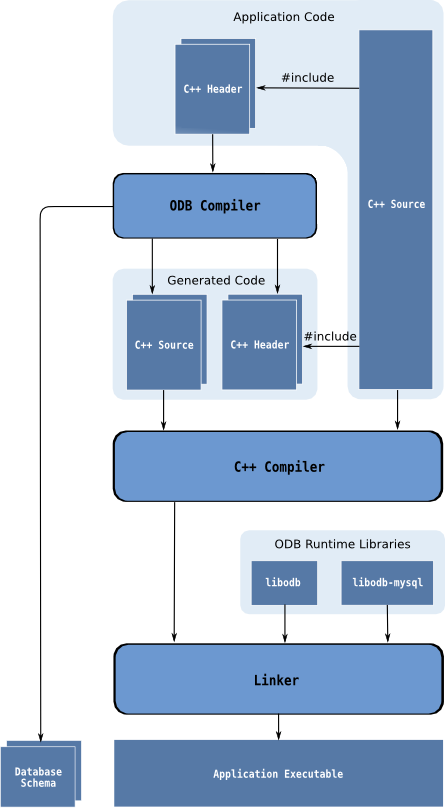
\includegraphics[width=0.4\textwidth]{odb-flow}
	\end{center}
	\caption{ODB Toolchain \cite{ODB_Manual}}
	\label{ODB-Flow}
\end{figure*}

\newpage

\subsubsection{Datenbankunabhängigkeit}
Durch die zusätzliche Abstraktionsschicht ist es einfacher die bestehende Persistenzschicht auf ein neues Datenbanksystem zu portieren.\\
Die umgesetzte Lösung ist weitestgehend frei von datenbankspezifischen Aufrufen, und benutzt ausschließlich die Schnittstelle des eingesetzten Object-Relational-Mappers.
Lediglich das User-Management, um ``Mitarbeiter`` auf Datenbankbenutzer abzubilden verwendet Datenbankspezifische SQL-Kommandos, die über ODB abgewickelt werden.

\subsubsection{Integration in das Buildsystem}
Um das Buildsystem (CMake) automatisch bei Veränderungen des Quellcodes alle für ODB benötigten Dateien generieren zu lassen, wird im Buildscript wie folgt vorgegangen:
\begin{enumerate}
\item Suchen aller Dateien die ODB spezifische Pragma-Definitionen beinhalten.
\item Erstellen einer Vorschrift um für jede so gefundene Datei den ODB-Compiler aufzurufen.
	Dabei werden auch die Abhängigkeiten der generierten Dateien korrekt in das Buildsystem eingefügt, so dass diese nur neu generiert werden, wenn tatsächlich Änderungen an der jeweiligen Eingangsdatei oder deren Abhängigkeiten vorhanden sind.
\end{enumerate}
Der entsprechende Auszug aus dem CMake Buildscript:\\
\lstset{language=clean}
Jeder zum Projekt gehörende C++ Header wird eingelesen und nach ODB-Pragma-Definitionen durchsucht:
\begin{lstlisting}
foreach( header ${EBPdb_headers} )
	file( READ ${header} headercontent )
	if( "${headercontent}" MATCHES "#pragma[ \t]+db[ \t]+object" )
\end{lstlisting}
Für jede gefundene Datei wird die generierte ODB-Datei zu den zu kompilierenden Quelldateien hinzugefügt:
\begin{lstlisting}
		get_filename_component( headerbase ${header} NAME_WE )
		set( EBPdb_sources ${EBPdb_sources} ${headerbase}-odb.cxx )
\end{lstlisting}
Damit der ODB-Precompiler den Quellcode korrekt parsen kann, müssen sämtliche verwendeten Include-Verzeichnisse bei dem Aufruf des Precompilers angegeben werden. Die Projekteinstellungen werden hierfür übernommen:
\begin{lstlisting}
		get_directory_property( odbincludes INCLUDE_DIRECTORIES )
		foreach( includedir ${odbincludes} )
			set( odbincludeargs ${odbincludeargs} -I${includedir} )
		endforeach( includedir )
\end{lstlisting}
Eine Regel zum Ausführen des Precompilers der der die Quellcode-Datei generiert wird erstellt (gleichzeitig werden auch alle weiteren benötigten Dateien erzeugt):
\begin{lstlisting}
		add_custom_command( OUTPUT ${headerbase}-odb.cxx ${headerbase}-odb.hxx ${headerbase}-odb.ixx ${headerbase}.sql
			COMMAND odb ${odbincludeargs} --database mysql --profile qt --generate-query --generate-schema ${header}
			DEPENDS ${header} )
	endif( "${headercontent}" MATCHES "#pragma[ \t]+db[ \t]+object" )
endforeach( header )
\end{lstlisting}

\newpage

\subsubsection{Datenbankschema}
\begin{figure*}[htp!]
	\begin{center}
		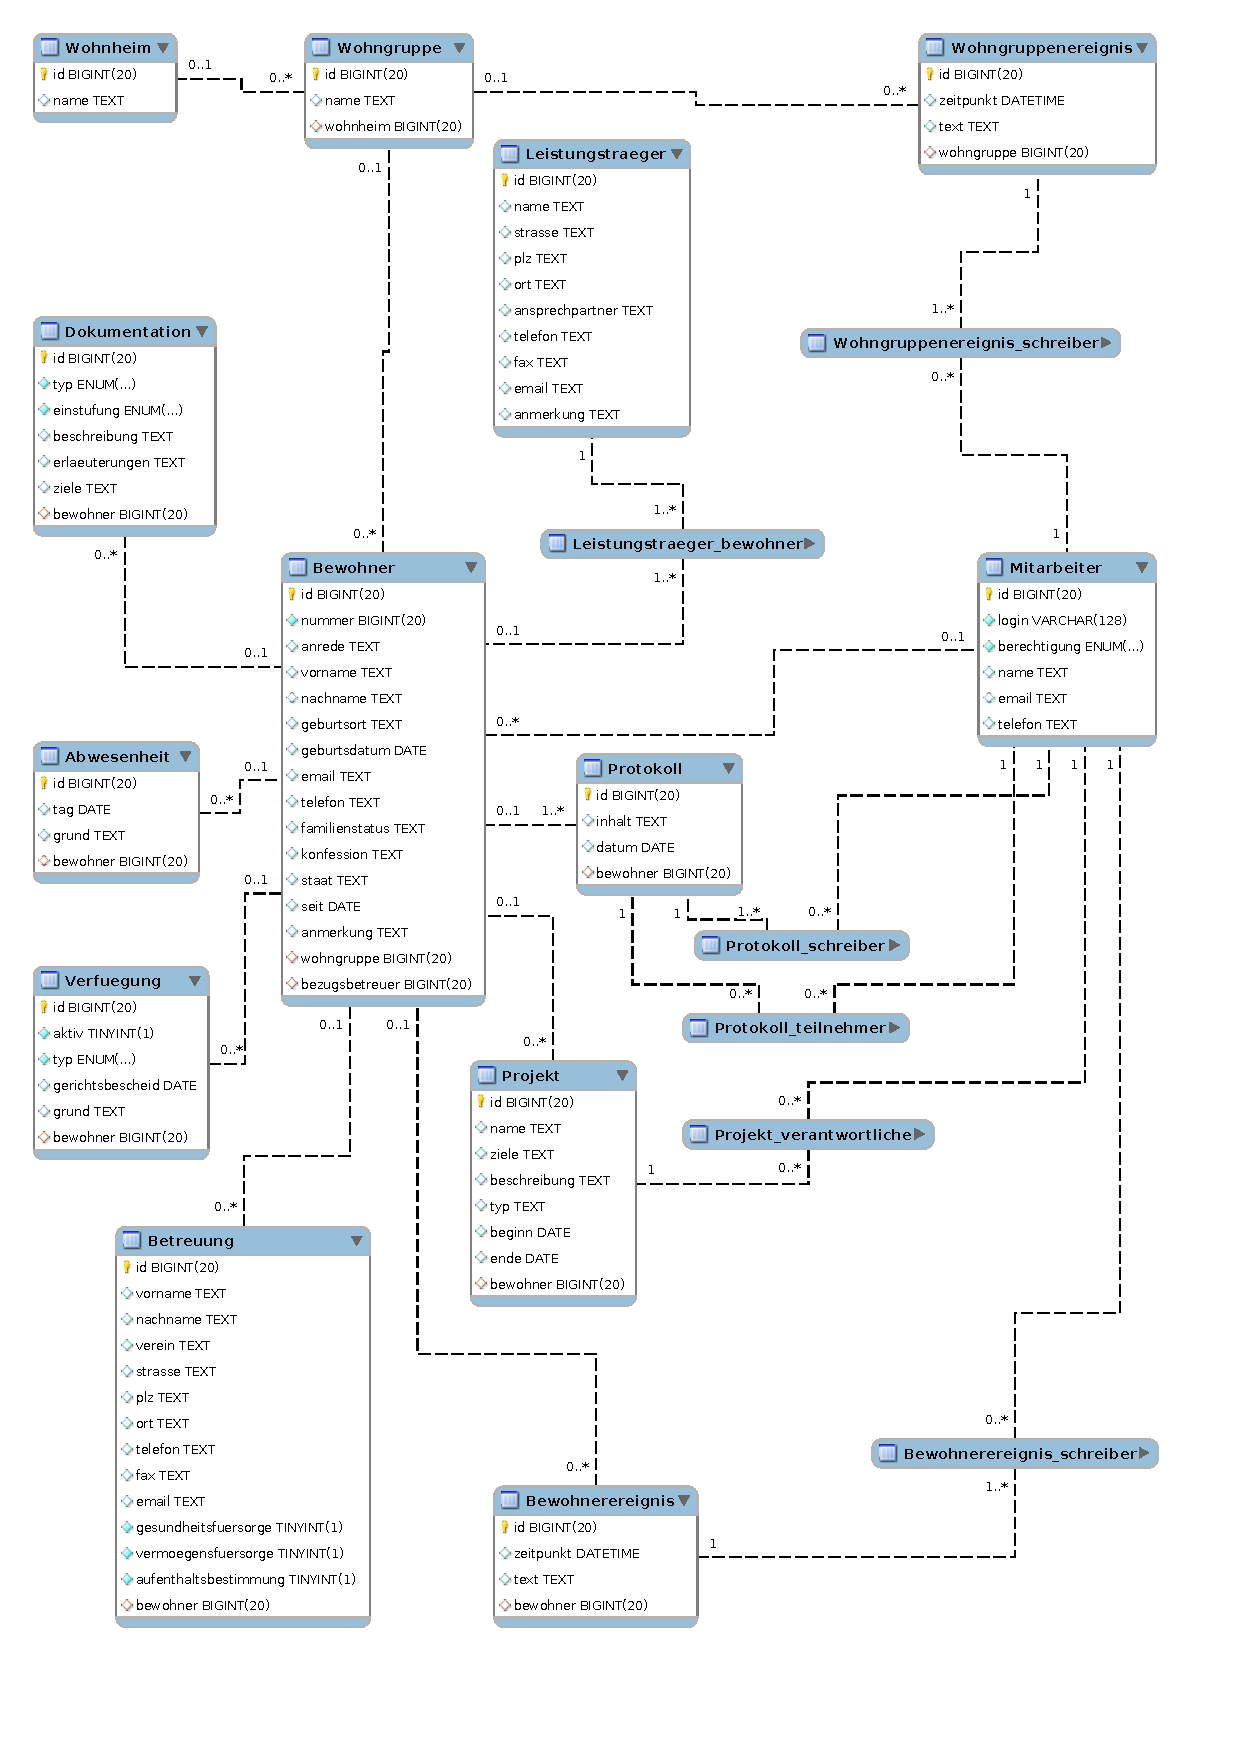
\includegraphics[width=0.93\textwidth]{scheme}
	\end{center}
	\caption{Datenbankschema als ER Diagramm}
	\label{ERDiagram}
\end{figure*}

\subsubsection{Abstraktion der Schnittstelle}
\lstset{language=c++}
Zweck der Bibliothek ist es die internen Abläufe des ORM Systems zu verbergen, und der Anwendung eine einfache, objektorientierte Schnittstelle zur Verfügung zu stellen.\\
Voraussetzung zur Verwendung der Bibliothek ist eine funktionierende Verbindung zur Datenbank:\\
\begin{lstlisting}
QSharedPointer<ebp::connection> connection =
	QSharedPointer<ebp::connection>
	(
		new ebp::connection( "LoginName", "DatenbankName", "localhost", 3306)
	);
connection->establish( "PasswortDesBenutzers" );
QSharedPointer<Mitarbeiter> mitarbeiter = connection->mitarbeiter();
\end{lstlisting}
Sollen neue Mitarbeiter auf die Datenbank zugreifen, kann mit\\
\begin{lstlisting}
QSharedPointer<ebp::Mitarbeiter> neuerMitarbeiter =
	QSharedPointer<ebp::Mitarbeiter>
	(
		new ebp::Mitarbeiter( "LoginName", ebp::Mitarbeiter::WohngruppenRecht, "Name" )
	);
neuerMitarbeiter->create( connection, "PasswortDesNeuenMitarbeiters" );
\end{lstlisting}
ein neuer Mitarbeiter in der Datenbank erstellen. Gleichzeitig wird auch ein neuer Datenbankbenutzer angelegt, der intern mit den Daten des Mitarbeiters verknüpft wird.
Der Datenbankbenutzer erhält dabei nur die Berechtigungen an den Datenbanktabellen, die er für seinen ''Rechtestatus`` benötigt.\\
\\
Analog zum Erstellen eines Mitarbeiters, lassen sich auch alle anderen Objekte der Bibliothek erzeugen:\\
\begin{lstlisting}
QSharedPointer<ebp::Bewohner> bewohner =
	QSharedPointer<ebp::Bewohner>
	(
		new ebp::Bewohner( 0 )
	);
bewohner->create( connection );
\end{lstlisting}
Veränderungen eines Objekts lassen sich mit der ''update``-Methode in der Datenbank sichern:\\
\begin{lstlisting}
bewohner->telefon( "0123456789" );
bewohner->update( connection );
\end{lstlisting}
Verknüpfungen lassen sich mit den jeweiligen ''link``-Methoden herstellen:\\
\begin{lstlisting}
ebp::Bewohner::linkBezugsbetreuer( bewohner,mitarbeiter);
ebp::Bewohner::linkWohngruppe( bewohner, wohngruppe);
bewohner->update( connection );
\end{lstlisting}
Dabei geht eine Verknüpfung immer von einer der Klassen aus - die andere ist das ''inverse`` Gegenstück.
Um die Verknüpfung persistent zu machen, muss immer die ''update``-Methode der Klasse verwendet werden, von der die Verknüpfung ausgeht.\\
Angelegte verknüpfungen lassen sich mit den verschiedenen ''load``-Methoden wieder laden:\\
\begin{lstlisting}
QList< QSharedPointer<ebp::Projekt> > projekte = bewohner->loadProjekte( connection );
\end{lstlisting}

\newpage

\subsection{Unit-Tests}

Unit-Tests, auch Komponententests genannt, sind sehr entwicklungsnahe Tests und sollen sicherstellen, dass die Erwartungen an eine Software erfüllt
werden können, indem Fehler vermieden werden.\\
''Das Testen von Software dient durch die Identifizierung von Defekten und deren anschließender Beseitigung zur Steigerung der Softwarequalität. Die 
Testfälle sollen so gewählt werden, dass sie weitgehend der späteren Benutzung der Software entsprechen. Die nachgewiesene Qualität des
Programmswährend der Tests entspricht dann der zu erwartenden Qualität während der späteren Benutzung\cite[S. 11]{Softwaretests}.''\\

Bei Unit-Tests werden einzelne Programmmodule isoliert von einander getestet. Dadurch sollen Einflüsse durch andere Softwarekomponenten ausgeschlossen
werden. Programmmodule müssen dabei aber nicht zwingendermaßen nur einzelne Klassen oder Funktionen sein \cite[Vgl. S. 11]{Softwaretests}. Bei der
\EBP erfolgt die Trennung in die Programmmodule libEBPdb und GUI. Für die Qualitätssicherung der GUI-Funktion wurden keine automatisierter Testcode
eingesetzt. Die korrekte Funktionalität der GUI wurde durch das regelmäßige Testen aller Masken durch einen Tester gewährleistet. Sollen auch diese
Aufgaben automatisiert werden, stellt Qt eine beschränkte API für User Interface Tests zur Verfügung. Darüber hinaus gibt es auch weitere
Drittanbieter für Tools und Frameworks zum automatisierten Testen von User Interfaces, wie z.B. TestComplete von Smart Bear. Diese Tests sind
allerdings äußerst aufwendig zu konfigurieren und zu pflegen.\\

Es wurden daher in erster Linie die libEBPdb mit Hilfe von automatisierten Unit-Tests getestet. Es sollte eine Testumgebung entworfen werden, die es
dem Entwickler ermöglicht nach einer Änderung im Quellcode mit Hilfe eines einzelnen Befehls überprüfen zu können, ob die libEBPdb als Gesamtheit noch
korrekt ausgeführt wird. Dazu wurde die Testumgebung mit Hilfe des Testtools CTest, ein Teil von CMake, in das Buildsystem integriert. Als Framework
für die eigentlichen Unit-Tests kommt die QTestLib, ein Teil von Qt, zum Einsatz. QTestLib bietet diverse Makros, die ein errechnetes Ergebnis mit dem
erwarteten Wert vergleichen und ein abweichendes Verhalten protokollieren. Dies ist die grundlegende Vorgehensweise bei einem Unit-Test. So
vergleicht der folgende Aufruf des Macros QCOMPARE den Rückgabewert einer Methode der Klasse ebp::Wohngruppe mit dem erwarteten Wert. Im Fehlerfall
wird der Rückgabewert und die Fehlerstelle protokolliert.
\begin{lstlisting}
QCOMPARE(wohngruppenEreignisList.at(i)->zeitpunkt(),QDateTime(QDate(2012,4,1),QTime(11,11)));
\end{lstlisting}



\newpage

\subsection{Eingesetzte Entwurfsmuster}
\subsubsection{Mediator Pattern - Der Text Transfer Agent}
Neben der Verwaltung von klienten- und wohngruppenspezifischen Daten ist die Überführung von Textstücken aus verschiedenen Teilen des
Dokumentationsprogramms die Hauptfunktion der \EBP. Diese Funktion wird im folgenden \textit{Text Transfer} genannt. \newline
Der \textit{Text Transfer} soll aus den Masken Bewohner$\rightarrow$Protokoll, Bewohner$\rightarrow$Projekt und Wohngruppe$\rightarrow$Gruppenbuch
erfolgen. Gespeichert werden die Textfragmente in den verschiedenen Feldern der Betreuungsplanung eines beliebigen Bewohners. Die Unterschiedlichkeit
der Quellen für die zu transferierende Textfragmente und die Variation an Zielfelder war die Schwierigkeit bei der Implementierung dieser
Funktionalität. Da die Anzahl an Objekten, die als Quelle dienen, im Programmverlauf stark variieren kann, muss der Lösungsansatz sehr flexibel
implementiert sein. Abbildung \ref{unstrukturiert} zeigt die Vielzahl an möglichen Kommunikationswegen zwischen den einzelnen Objekten.\\
\begin{figure*}[htp!]
	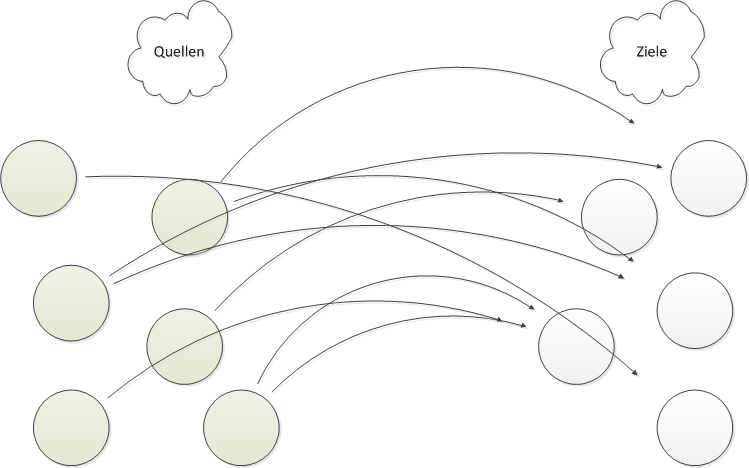
\includegraphics[width=0.8\textwidth]{unmediated}
	\caption{Kommunikationswege zwischen Objekten}
	\label{unstrukturiert}
\end{figure*}
Um nicht jeden Kommunikationsweg einzeln verwalten zu müssen, wurde der \textit{Text Transfer} in Form des Mediator Patterns entworfen. Den Zweck
eines Mediators definiert GAMMA wie folgt: \\
``Define an object that encapsulates how a set of objects interact. Mediator promotes loose coupling by keeping objects from reffering to each other explicitly, 
and it lets you vary their interaction independently \cite[S. 273]{Entwurfsmuster}.''\\
\\
\textbf{Beteiligte Objekte\cite[S. 277]{Entwurfsmuster}:}
\begin{enumerate}
	\item Eine Instanz des TextTransferAgent als konkreter Mediator. Auf eine abstrakte Mediatorklasse wurde auf Grund des klar definierten Aufgabengebiets verzichtet.
	\begin{enumerate}
		\item Implementiert die Interaktion zwischen den verschiedenen Kollegen.
		\item Kennt alle zu verwaltenden Kollegenobjekte.
		\item Deklaration der Mediatorklasse TextTransferAgent:
		\begin{lstlisting}
class TextTransferAgent : public QFrame
{
    Q_OBJECT

public:
    explicit TextTransferAgent(QList<TextTransferInterface *>Interfaces,const SessionContext &context, QWidget *parent = 0);
    ~TextTransferAgent();
    void registerNewInterface(TextTransferInterface *newInterface);

private slots:
    void on_bewohnerBox_currentIndexChanged(int index);
    void on_losButton_clicked();
    void on_helpButton_clicked();

private:
    const SessionContext &_context;
    Ui::TextTransferAgent *ui;
    QSharedPointer< ebp::Bewohner > selectedBewohner;
    QList < QSharedPointer < ebp::Dokumentation > > dokus;
    QList<TextTransferInterface *> textInterfaces;
};
		\end{lstlisting}
	\end{enumerate}
	\item Beliebig viele Instanzen von Klassen, die das TextTransferInterface implementiert haben als Kollegen.
	\begin{enumerate}
		\item Jeder Kollege kennt das Mediatorobjekt.
		\item Möchte ein Kollege mit einem anderen kommunizieren, tut er dies über den Mediator.
		\item Die Kommunikation zwischen den Kollegen ist in dieser Implementierung unidirektional. Klassen, die das TextTransferInterface implementiert haben dienen stets 
			als Quelle für den Texttransfer. Als Ziel für den Texttransfer stehen dem Meditor über das aktive Bewohner Objekt alle Instanzen der Betreuungsplanung zur Verfügung.
		\item Deklaration des Kollegeninterfaces TextTransferInterface:
		\begin{lstlisting}
class TextTransferInterface
{
public:
    virtual TextTransferInformation getSelectedText()=0;
};
		\end{lstlisting}
	\end{enumerate}
\end{enumerate}
Abbildung \ref{strukturiert} zeigt die Kommunikationswege eines Texttransfers zwischen den einzelnen Objekten, koordiniert durch ein Mediatorobjekt. 
\begin{figure*}[htp!]
	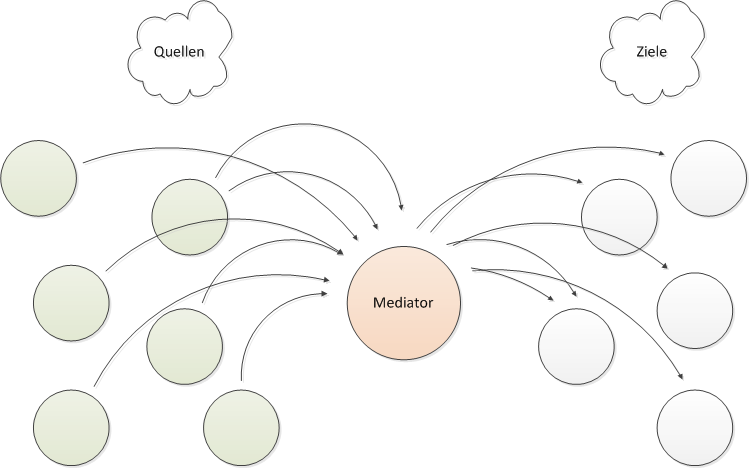
\includegraphics[width=0.8\textwidth]{mediated}
	\caption{Kommunikationswege zwischen Objekten, koordiniert durch einen Mediator}
	\label{strukturiert}
\end{figure*}
\subsubsection{Observer Pattern - Signal Slot Konzept}
Ein klassisches Konzept zur Kommunikation zwischen Objekten stellen \textit{Events} und \textit{Eventhandler} dar. Dieses Konzept ist allerdings nicht typsicher und unflexibel, da es für ein \textit{Events} auch nur einen \textit{Eventhandler} geben kann\cite[S. 32]{Qt4}. Qt hingegen nutzt zur Kommunikation zwischen Objekten das \textit{Signal Slot Konzept}, das wie ein Observer Pattern aufgebaut ist. GAMMA beschreibt das Observer Pattern wie folgt: \\
"Define a one-to-many dependency between objects so that when one object changes state, all its dependents are notified and updated automatically\cite[S. 293]{Entwurfsmuster}."\\
Qt realisiert dies, indem Funktionen einer Klasse durch das Schlüsselwort \textit{Slot} gekennzeichnet werden können. Diese \textit{Slots} werden mit einem \textit{Signal} verbunden und sind damit als \textit{Observer} zu betrachten. Das \textit{Subject} ist ein Funktionsprototyp, der durch das Schlüsselwort \textit{Signal} gekennzeichnet wird. Dieser Prototyp wird nicht implementiert. GAMMA beschreibt diese Beziehung folgendermaßen:\\
''The Subject is the publisher of notifications. It sends out these notifications without having  to know who its observers are. Any number of observers can subscibe to receive notifications\cite[S. 294]{Entwurfsmuster}."\\
Verbunden wird ein \textit{Signal} mit einem \textit{Slot} durch den Aufruf der statischen Methode QObject::connect(). \textit{Signal} und \textit{Slot} müssen dabei die gleichen Argumente besitzen. Dadurch wird die Typsicherheit gewährleistet. Allerdings sind die Schlüsselworte \textit{Signal} und \textit{Slot} kein reines C++. Klassen die sich diesem Konzept bedienen müssen daher durch den \textit{Meta Object Compiler (MOC)} in Standard-konformes C++ verwandelt werden\cite[Vgl. S. 51]{Qt4}.
\EBP bedient sich dieses Konzepts an vielen Stellen. Der Anmeldevorgang soll hier als Beispiel dienen. Die Anmeldung an dem Client erfolgt auf einer Maske, die durch die Klasse LoginForm beschrieben wird. Diese Klasse definiert auch ein eigenes \textit{Signal} \textit{validLogin()}:
\begin{lstlisting}
class LoginForm : public QWidget
{
    ...
signals:
    void validLogin(QSharedPointer<ebp::Mitarbeiter> newMitarbeiter, QSharedPointer<ebp::connection> newConnection);
    ...
};
\end{lstlisting}
Die Klasse MainWindow definiert den dazu passenden \textit{Slot}, der nach einer erfolgreichen Anmeldung den Client initialisiert:
\begin{lstlisting}
class MainWindow : public QMainWindow
{
    ...
private slots:
    void validLogin(QSharedPointer<ebp::Mitarbeiter> newMitarbeiter, QSharedPointer<ebp::connection> newConnection);
    ...
};
\end{lstlisting}
Durch dieses Konzept der losen Kopplung könnten bei Bedarf weitere \textit{Slots} an ein erfolgreiches Anmelden angekoppelt werden, ohne auf den bereits bestehenden \textit{Slot} zum initialisieren des Clients Einfluss zu nehmen.
\subsubsection{Model/View Pattern - Datenvisualisierung}
Das Entwurfsmuster Model/View oder auch Model/View/Controller ist ein klassisches Entwurfsmuster der Softwareentwicklung und beschreibt, wie die Datenhaltung, die Visualisierung der Daten und die Interaktion mit dem Benutzer in verschiedenen Komponenten realisiert wird. Ziel dieses Entwurfsmusters ist es, flexiblen und wiederverwendbaren Programmcode zu entwickeln.
Das Framework Qt bietet die Variante des Model/View Entwurfsmusters an. Dabei werden Der Controller und der View in der selben Komponente realisiert. Dies vereinfacht die Handhabung, ermöglicht aber immernoch ein Trennen der Datenhaltung und der Visualisierung der Daten \cite[Vgl.]{QtModelView}.
Qt bietet Abstrakte Klassen für ein Table-, List- oder Treemodel an, um grundlegene Funtionalitäten für die entsprechenden Views vorzugeben. Sind diese Ansätze nicht flexibel genug, kann QAbstractItemModel implementiert werden. Um die Mitarbeiterobjekte in einem Tableview darstellen zu können, wurde ein einfaches Model mit Hilfe von QAbstractTableModel implementiert:
\begin{lstlisting}
class EmployeeTableModel : public QAbstractTableModel
{
    Q_OBJECT
    QList < QSharedPointer < ebp::Mitarbeiter > > EmployeeList;
public:
    explicit EmployeeTableModel(QList < QSharedPointer < ebp::Mitarbeiter> > employees, QObject *parent = 0);
    
    // Überschriebene Funktion. Liefert dem View die Anzahl an Zeilen    
    int rowCount(const QModelIndex &parent) const;

    // Überschriebene Funktion. Liefert dem View die Anzahl an Spalten
    int columnCount(const QModelIndex &parent) const;

    // Überschriebene Funktion. Liefert dem View die Daten.
    QVariant data(const QModelIndex &index, int role) const;

    // Überschriebene Funktion. Liefert dem View die Überschriften.
    QVariant headerData(int section, Qt::Orientation orientation, int role);
    QSharedPointer < ebp::Mitarbeiter> getMitarbeiter(int index);
    void addMitarbeiter(QSharedPointer<ebp::Mitarbeiter> newMitarbeiter);
};
\end{lstlisting}
Dieses Model kann in verschiedenen Tableviews verwendet werden. Die Views können sich stark von einander unterscheiden. Über die überschriebenen Funktionen von QAbstractTableModel wird sichergestellt, dass der View auf die richtigen Daten zugreift.
\newpage
